% NOAOPROP.TEX -- template for NOAO STANDARD telescope proposals.
% Revised for the 2018B semester (August - January 2018)
% For later semesters, the current form may be obtained from our Web
% page at http://www.noao.edu/noaoprop/noaoprop.html

% DEADLINE FOR SUBMISSIONS: 11:59pm MST MONDAY APRIL 2 

% This form can NOT be used to submit Gemini proposals.  Please
% see:   http://www.noao.edu/noaoprop/help/pit.html

% This LaTeX template has been returned to you upon request through
% our Web-based proposal form.  The template has been customized for
% you based on the run information that you entered via the Web form.
% As an option you may complete this form locally and submit it by
% email following the instructions below.  If the run information is
% incomplete you should go back to the Web form, complete all the
% suggested run information and then obtain another customized 
% template before proceeding. 
%
% WEB FORM SUBMISSION:
% If you have not modified this document locally, we encourage web
% submissions using the "Proposal Submission" button on the web
% proposal form.  Be sure to click on the second prompt on the
% following page to complete submission.   Skip to step #3 below
% for some additional information.
%
% FILE UPLOAD SUBMISSION:
% If you have modified this document locally and are ready to submit, 
% you do not need to return to the web form.  Instead, you may submit
% this template and figure files by following the instructions 
% below.
%
%   1. Before submitting this form electronically, run it through latex
%      and print it out to make certain that it looks the way that you
%      wish the review panel to see it.
%   
%   2. Upload THIS file (NOT the PostScript or PDF version) and
%      all figures on the web at http://www.noao.edu/noaoprop/submit/
%
%   3. If the proposal is a thesis or if the principal investigator is a
%      a graduate student, the student's faculty advisor must complete
%      the online form at http://www.noao.edu/noaoprop/thesis/
%      This form should be completed within two business days after the
%      deadline.  Graduate students proposing thesis observations should
%      consult NOAO policies concerning thesis programs and travel support.
%
%   4. QUESTIONS?  If you have questions about submitting your proposal
%      send email to noaoprop-help@noao.edu.  Information about
%      instrumentation can be found at the NOAO Web 
%      site at http://www.noao.edu/noaoprop/noaoprop.html.  Specific 
%      instrumentation or facility questions for CTIO or KPNO
%      can also be sent to the respective sites at ctio@noao.edu, 
%      and kpno@noao.edu
%      Gemini questions can be  emailed to the US mirror scientists 
%      at nssc@noao.edu.
%
%   5. When your proposal is received at NOAO you will be sent an
%      automatic email message verifying its receipt along with a
%      proposal ID number.  If you do not receive this message within
%      15 minutes of the time you sent your proposal send email to
%      noaoprop-help@noao.edu for assistance.  You may track your
%      proposal processing by the proposal ID number at the following
%      web page:   https://www.noao.edu/cgi-bin/noaoprop/propstatus
% ___________________________________________________________________
% THE FORM STARTS HERE
%

% Please do not modify or delete this line.
\documentclass[11pt]{article}
\usepackage{nprop30}
\usepackage{graphicx}
\usepackage{longtable}
\usepackage{natbib}
\usepackage{hyperref}
\hypersetup{colorlinks = true, citecolor = blue, linkcolor = magenta, urlcolor = magenta}


% Please do not modify or delete this line.
\begin{document}

% Uncomment the following line and enter a previous semester and ID
% (e.g. 01B-0987) if you wish to flag this proposal as a resubmission
%\pastid{}

% Please do not modify or delete this line.
\proposaltype{Standard}
% Do not delete the following uncommented line which is required for Gemini 
% proposals.  This line indicates whether or not the proposal is being 
% submitted to multiple partner countries - only "yes" or "no" is valid.
\geminidata{mpartners}{no}

%%%%%%%%%%%%%%%%%%%%%%%%%%%%%%%%%%%%%%%%%%%%%%%%%%%%%%%%%%%%%%%%%%%%%

% SCIENTIFIC CATEGORIES
%
% Please select a "scientific category" that best describes your
% program by uncommenting only ONE of the selections below.  Your
% \sciencecategory selection will be used to assign a review panel to
% your proposal.  DO NOT MODIFY THE SELECTION YOU UNCOMMENT.  A
% description of each of these categories is available on our Web page
% at https://www.noao.edu/noaoprop/help/scicat.html

% EXTRA-GALACTIC LIST (do not uncomment this line)
%\sciencecategory{Active Galaxies}
%\sciencecategory{Cosmology}
%\sciencecategory{Large Scale Struc.}
%\sciencecategory{Clusters of Galaxies}
%\sciencecategory{High Z Galaxies}
%\sciencecategory{Low Z Galaxies}
%\sciencecategory{Resolved Galaxies}
%\sciencecategory{Stellar Pops (EGAL)}
%\sciencecategory{EGAL - Other}

% GALACTIC/LOCAL GROUP LIST (do not uncomment this line)
%\sciencecategory{Star Clusters}
%\sciencecategory{Stellar Pops (GAL)}
%\sciencecategory{HII Reg., PN, etc.}
%\sciencecategory{ISM}
%\sciencecategory{Star Forming Regions}
%\sciencecategory{Young Stellar Obj.}
%\sciencecategory{Massive Stars}
%\sciencecategory{Low Mass Stars}
%\sciencecategory{Stellar Remnants}
\sciencecategory{Galactic - Other}

% SOLAR SYSTEM LIST (do not uncomment this line)
%\sciencecategory{Kuiper Belt Objects}
%\sciencecategory{Small Bodies \& Moons}
%\sciencecategory{Planets}
%\sciencecategory{Extrasolar Planets}
%\sciencecategory{Solar System - Other}

%%%%%%%%%%%%%%%%%%%%%%%%%%%%%%%%%%%%%%%%%%%%%%%%%%%%%%%%%%%%%%%%%%%%%%

% TITLE
%
% Give a descriptive title for the proposal in the \title command.
%
% Note that a title can be quite long; LaTeX will break the title into
% separate lines automatically.  If you wish to indicate line breaks
% yourself, do so with a `\\' command at the appropriate point in
% the title text.  Use both upper and lower case letters (NOT ALL CAPS).

\title{Probing Short Duration Stellar Variability with Star Trail Images of Four K2 Fields}


%%%%%%%%%%%%%%%%%%%%%%%%%%%%%%%%%%%%%%%%%%%%%%%%%%%%%%%%%%%%%%%%%%%%%%

% ABSTRACT
%
% Give a general abstract of the scientific justification appropriate
% for a non-specialist.  Write between the \begin{abstract} and 
% \end{abstract} lines.  Limit yourself to approximately 175 words.
% Abstracts of accepted proposals will be made publicly available.

% DO NOT remove the \begin{abstract} and \end{abstract} lines.

\begin{abstract}
\citealt{2018arXiv180806977T} demonstrated, using high fidelity ray-tracing simulations, that star trail images enable wide-field ground-based telescopes to resolve stellar variability down to a time scale of 10 milliseconds. We request half a night with the Dark Energy Camera on the Blanco 4-m telescope to take star trail images of four K2 fields to validate this method, characterize its performance, and detect new sources of stellar variability. The 270 square degree survey will be the first of its kind and will add a new dimension to our understanding of over 10,000 sources.

% improve our understanding of the variable universe on short time scales. 
%short duration stellar variability composition of the universe.
\end{abstract}

%%%%%%%%%%%%%%%%%%%%%%%%%%%%%%%%%%%%%%%%%%%%%%%%%%%%%%%%%%%%%%%%%%%%%%

% SUMMARY OF OBSERVING RUNS REQUESTED
%
% List a summary of the details of the observing runs being requested,
% for UP TO SIX runs.  The parameters for each run are segregated
% between \begin{obsrun} and \end{obsrun} lines.  Please be sure
% that the information is isolated properly for each run.
%
%   \begin{obsrun}
%   \telescope{}        % For example, \telescope{KP-4m}
%   \instrument{}       % For example, \instrument{ECHUV + T2KB}
%   \numnights{}        % For example, \numnights{6}
%   \lunardays{}        % For example, \lunardays{grey}
%   \optimaldates{}     % For example, \optimaldates{Sep - Nov}
%   \acceptabledates{}  % For example, \acceptabledates{Aug - Jan}
%   \end{obsrun}
%
% The following telescope identifiers MUST be used in the \telescope{}
% field.  Some of the telescope identifiers must include an observatory
% code as well.
%
% CTIO: CT-4m, SOAR, CT-1.3m, CT-0.9m
% KPNO: WIYN, KP-0.9m
% AAO: AAT
% LCO: LCO-2m, LCO-1m
% CHARA: CHARA
%
% Select the instrument and detector identifiers from the list on our
% Web page at https://www.noao.edu/noaoprop/help/facilities.html.
% The correct codes MUST be used to ensure your correct
% instrument + detector combination.
%
% \numnights should give the number of nights of the run (for queue
% observations, use fractional 10-hour equivalent nights, e.g.
% 3 hours = 0.3 nights).  Formats such as 5x0.5 are acceptable.
%
% \lunardays should contain the word "darkest", "dark", "grey", or
% "bright", which in turn reflects the number of nights from new moon
% where darkest<=3, dark<=7, grey<=10, bright<=14.  Particular lunar 
% phase requirements dictated by the science program (e.g., "<=12", 
% "+9, -6", or "full moon more than 2 hours away from Taurus") should
% be noted in the "scheduling constraints or non-usable dates" section 
% below.
%
% \optimaldates should contain the range of OPTIMAL months, as shown 
% below.
%
% \acceptabledates should give the range of ACCEPTABLE months (i.e.,
% you would not accept time outside those limits).
% NOTE THAT DUE TO INSTRUMENT BLOCKING RESTRICTIONS YOU SHOULD MAKE 
% THIS RANGE AS GENEROUS AS POSSIBLE.
%
% For QUEUE-SCHEDULED observations, you may set the date range to the 
% full semester range and set \lunardays to the brightest moon your
% observations could tolerate if the program were scheduled classically.
%
% To enter the acceptable and optimal date ranges, please use two
% dash-separated months with 3-letter abbreviations for the month
% (Jan, Feb, Mar, Apr, May, Jun, Jul, Aug, Sep, Oct, Nov, Dec).
% For example:  \optimaldates{Nov - Dec}.
% We appreciate your help in not using vague range specifications
% like "October dark run" or "mid-January" which will require human
% intervention.
%
% FOR LONGTERM STATUS PROPOSALS SPECIFY ONLY THE RUNS FOR THE CURRENT
% SEMESTER, AND NOT FOR ANY SUBSEQUENT SEMESTERS.

% DO NOT remove any of the \begin{obsrun} and \end{obsrun} blocks, 
% even if the blocks are empty.

\begin{obsrun}
\telescope{CT-4m}
\instrument{DECam}
\numnights{0.5}
\lunardays{grey}
\optimaldates{May - July}
\acceptabledates{May - July}
\end{obsrun}

\begin{obsrun}
\telescope{}
\instrument{}
\numnights{}
\lunardays{}
\optimaldates{}
\acceptabledates{}
\end{obsrun}

\begin{obsrun}
\telescope{}
\instrument{}
\numnights{}
\lunardays{}
\optimaldates{}
\acceptabledates{}
\end{obsrun}

\begin{obsrun}
\telescope{}
\instrument{}
\numnights{}
\lunardays{}
\optimaldates{}
\acceptabledates{}
\end{obsrun}

\begin{obsrun}
\telescope{}
\instrument{}
\numnights{}
\lunardays{}
\optimaldates{}
\acceptabledates{}
\end{obsrun}

\begin{obsrun}
\telescope{}
\instrument{}
\numnights{}
\lunardays{}
\optimaldates{}
\acceptabledates{}
\end{obsrun}


% If there are scheduling constraints or non-usable dates for any of
% the runs specified, (i.e., other than the default lunar phase 
% requirements or when your object is up) please give the dates by 
% filling in the curly braces in \unusabledates{}.  Note here if you 
% are requesting runs in an "either/or" situation, e.g. run 1 or run 2, 
% but not both. This is also the place to advise us of any special 
% constraints which affect the scheduling of your observing run (e.g. 
% "schedule run #1 before run #2" or "run dates must be coordinated 
% with HST observations").
% 
% Please limit your text to six lines on the printed copy.

\unusabledates{We have no scheduling constraints.}

%%%%%%%%%%%%%%%%%%%%%%%%%%%%%%%%%%%%%%%%%%%%%%%%%%%%%%%%%%%%%%%%%%%%%%%

% INVESTIGATOR'S (PI AND CoI) INFORMATION BLOCKS
%
% Please give the PI's name (first name first followed by middle
% initial and last name), affiliation, department and complete mailing
% address, as well as an email address.  Also give a complete phone
% number, and a number for a fax machine if you have access to one.
% You must also indicate the principal investigator's status with one
% of the one-letter codes inside the \invstatus{} curly braces, as
% indicated below.
%
% The affil{}, \department{}, \address{} (use a comma separate list as
% needed), \city{}, \state{}, \zipcode{}, and \country{} (for non-US
% addresses) fields will be used together as your full postal mailing
% address.  Please be sure this information is complete.  Note that
% some institutions will not deliver postal mail if a department is
% not included in the postal mailing address.  Non-US addresses should
% include the country and any local postal codes.
%
% The fax number does not print on the form.
%
% For each CoI please include a name, affiliation, email address and
% investigator's status within the \begin{CoI} and \end{CoI} lines.
%
% For each \invstatus{} field, please fill in the appropriate
% investigator status code from the following list.  If the investigator
% is a graduate student, indicate "T" if THIS proposal is related to a
% thesis project, or "G" otherwise.  This code should represent the
% status of the individuals at the time of the proposal submission.
% This information is necessary to assist us with our required reporting
% to the NSF.
%
% \invstatus{P} % investigator has obtained PhD or equivalent
% \invstatus{T} % investigator is grad student, proposal is thesis
% \invstatus{G} % investigator is grad student, proposal not thesis
% \invstatus{U} % investigator is an undergraduate student
% \invstatus{O} % investigator has other status (none of the above)
%
% DO NOT remove the \begin{PI} and \end{PI}.  Only one individual's
% name per \name field is allowed.
%
% Investigator names will now appear on page 2 of the printed proposal.
% Do not remove this line.
\investigators

\begin{PI}
\name{David Thomas}
\affil{Stanford University}
\department{Institute for Computational and Mathematical Engineering}
\address{475 Via Ortega}
\city{Stanford}
\state{California}
\zipcode{94305}
% \country{United States}
\email{dthomas5@stanford.edu}
\phone{760-525-6973}
\fax{None}
\invstatus{G}
\end{PI}

\begin{CoI}
\name{Steven Kahn}
\affil{Stanford University}
\email{skahn@slac.stanford.edu}
\invstatus{P}
\end{CoI}

\begin{CoI}
\name{Krista Lynne Smith}
\affil{Stanford University}
\email{klynne@stanford.edu}
\invstatus{P}
\end{CoI}

\begin{CoI}
\name{Robert Blum}
\affil{National Optical Astronomy Observatory}
\email{rblum@noao.edu}
\invstatus{P}
\end{CoI}

\begin{CoI}
\name{Zeljko Ivezic}
\affil{University of Washington}
\email{ivezic@astro.washington.edu}
\invstatus{P}
\end{CoI}

\begin{CoI}
\name{Colin Burke}
\affil{University of Illinois Urbana-Champaign}
\email{colinjb2@illinois.edu}
\invstatus{G}
\end{CoI}



%\begin{CoI}
%\name{}
%\affil{}
%\email{}
%\invstatus{}
%\end{CoI}


%%%%%%%%%%%%%%%%%%%%%%%%%%%%%%%%%%%%%%%%%%%%%%%%%%%%%%%%%%%%%%%%%%%%%%

% In the following "essay question" sections, the delimiting pieces of
% markup (\justification, \expdesign, etc.) act as LaTeX \section*{}
% commands.  If the author wanted to have numbered subsections within
% any of these, LaTeX's \subsection could be used.
%
% DO NOT REDUCE THE FONT SIZE, and do not otherwise fiddle with the
% format to get more on a page.  We will reset any changes back to the
% default font.

% SCIENTIFIC JUSTIFICATION
%
% Give the scientific justification for the proposed observations.
% This section should consist of paragraphs of text followed by any
% references and up to three figures and captions.  Be sure to include
% overall significance to astronomy.  THE SCIENTIFIC JUSTIFICATION
% SHOULD BE LIMITED TO ONE PAGE (the review panels have requested that
% we not send them more than one page), with up to two additional pages
% for references, figures (no more than three), and captions. 

% If you wish to use our "reference" environment, follow the following
% example (journal commands are compatible with AASTeX v4.0):
%
% \begin{references}
% \reference Armandroff \& Massey 1991 \aj, 102, 927.
% \reference Berkhuijsen \& Humphreys 1989 \aap, 214, 68.
% \reference Massey 1993 in Massive Stars: Their Lives in the 
% Interstellar Medium (Review), ed. J. P. Cassinelli and E. B. 
% Churchwell, p. 168.
% \reference Massey \& Armandroff 1999, in prep.
% \end{references}

%
% Only EPS figures may be included with your proposal.  In order to
% include an EPS plot, you should use the LaTeX "figure" environment.
% The plot file is included with the \plotone{FILENAME} command; two
% side-by-side plot files can be included by typing
% \plottwo{FILENAME1}{FILENAME2}.  Use \caption{} to specify a caption.
% The \epsscale{} command can be used to scale \plotone plots if they
% appear too large on the printed page.  Contact us if you have any
% figure questions or encounter any problems with figures
% (noaoprop-help@noao.edu).
%
% \begin{figure}
% \epsscale{0.85}
% \plotone{sample.eps}
% \caption{Sample figure showing important results.}
% \end{figure}
%
% If you need to rotate or make other transformations to a figure, you
% may use the \plotfiddle command:
% \plotfiddle{PSFILE}{VSIZE}{ROTANG}{HSCALE}{VSCALE}{HTRANS}{VTRANS}
% \plotfiddle{sample.eps}{2.6in}{-90.}{32.}{32.}{-250}{225}
% where HSCALE and VSCALE are percentages and HTRANS and VTRANS are
% in PostScript units, 72 PS units = 1 inch.
%
% Note that the Web form provides several useful and simple figure 
% options.

\sciencejustification
% The Kepler K2 mission is a sequence of 80-day continuous observing campaigns of fields distributed around the ecliptic plane. For each field, K2 provides state of the art photometry for thousands of targets. The extensive time series data has propelled scientific investigation of a wide range of astrophysical phenomena. Seeking further insights, astronomers have engaged in follow up observations of these fields on other telescopes, including in the near infrared and x-ray regimes. High time resolution imaging, or sub-second photometry, however, is absent from this data ecosystem. Imaging the universe on short time scales can bolster the investigation of energetic phenomena from compact stellar remnants such as black holes, neutron stars, and white dwarfs; to two star systems such as cataclysmic variables, eclipsing binaries, and X-ray binaries; to extra-solar planets and brown dwarfs.

% The universe is teaming with phenomena that manifests on short time scales but that is dificult to image. A wide range of energetic phenomena from compact stellar remnants such as black holes, neutron stars, and white dwarfs; to two star systems such as cataclysmic variables, eclipsing binaries, and X-ray binaries; to extra-solar planets and brown dwarfs is intriguing to examine on short time scales. 

\subsection*{Probing Short Duration Stellar Variability with Star Trails}


Time domain astronomy has now begun in earnest and is revolutionizing many fields, especially using large surveys capable of collecting light curves en masse \citep{2012IAUS..285..141D}. However, almost none of these surveys is performing optical monitoring at less than a few minute timescales, omitting a variability regime that we know to be important for studying phenomena ranging from compact stellar remnants to trans-Neptunian objects: sub-second photometry. \citealt{2018arXiv180806977T} presented a new method and demonstrated, through high fidelity ray-tracing simulations, that it is capable of collecting such light curves for thousands of objects at a time. We propose using the Dark Energy Camera (DECam) on the Blanco 4-m telescope to validate this method and to provide sub-second photometry for four strategically chosen K2 fields (shown in Figure \ref{fig:1}).


% Charge-Coupled Devices (CCDs), the detector of choice for optical astronomy, take around 10 seconds to read out. This limits the time resolution of conventional telescopes. Dedicated instruments using special frame transfer and electron multiplying CCDs have achieved time resolution in tens of milliseconds on a 5 arcsecond field of view (Dhillon et al. 2007, 2014, 2016; Harding et al. 2016). While these instruments are sufficient for studying individual sources of variability, they are not well-suited for large surveys or searching for new sources of variability. In Thomas \& Kahn (2018), we present a technique that allows existing wide-field telescopes to achieve comparable time resolution. We propose using the Dark Energy Camera (DECam) on the Blanco 4-m telescope to validate this method and to provide sub-second photometry for four strategically chosen K2 fields.

% \subsection*{Exploring the Variable Universe on Short Time Scales}
Our method is comprised of operational and image processing components. The operational component is to take star trail images. A simulated DECam star trail image is shown in Figure \ref{fig:2}. The authors of \citealt{1986PASP...98..802H} realized that each trail serves as a light curve for its corresponding source and facilitates high time resolution photometry. We have trained a deep neural network to identify stellar variability in simulated star trail images from the Large Synoptic Survey Telescope (LSST). The network detection efficiency on tophat-like flares is shown in Figure \ref{fig:3}. We are preparing the next generation of our network for DECam. 

DECam's wide field of view and superb resolution make it the best instrument to validate our method with \citep{2015AJ....150..150F}. The 2.2 degree field of view captures many sources simultaneously and allows us to survey the sky around 700 times faster than existing high time resolution instruments \citep{2007MNRAS.378..825D}. The wide field is complemented by a 570 Megapixel camera and 0.26 arcsecond pixel scale which mean that a trailing source will spend approximately $17 / \cos(\delta)$ milliseconds over each pixel, leading to excellent time resolution. After validating and further refining our method on DECam we hope to employ it during the commissioning of the LSST. 

The proposed survey is the first of its kind and will add a new dimension to our knowledge of the four chosen K2 fields. Scanning the sky for M-dwarf flares will allow us to constrain their frequency, correlate them with cluster properties, and compare high time resolution photometry of the flare up with numerical simulations \citep{2017ApJ...849...36Y,2017ApJS..232...26V}. Occultations from trans-Neptunian objects would allow us to detect new structures in the solar system, in particular the small Kuiper Belt Objects that are of particular theoretical interest and which produce occultations lasting for tens of milliseconds \citep{2000Icar..147..530R,2013AJ....146...14Z}. Perhaps the most intriguing possibility is that we will discover new sources of variability. 

%\citep{2017arXiv170705167S}


% The proposed survey will get star trails over a wide swathe of sky. This will allow us to accurately measure M-dwarf flares and constrain their frequency across the X,Y,Z open clusters. TNO occultations can also help us discover new TNO objects. The most intriguing possibility is discovering a new source of variability.


% Kepler fields have been extensively studied. Often times there are synergies between these studies that complement each other. However no mechanism to study short term optical variability. 

% Most of our understanding of what causes a star to flare is based on observations of the only star near enough to examine in detail — the Sun. But in learning from a sample size of one, a challenge arises: we must determine which conclusions are unique to the Sun (or Sun-like stars), and which apply to other stellar types as well.

% Stellar flares are good observational tracers of magnetic
% activity in low-mass stars (especially M dwarfs), since the
% intense release of flare energy is necessarily related to magnetic
% fields that are generated by dynamo process as on the Sun.


% compact object physics that manifests on short time scales. Charge-Coupled Devices (CCDs), the detector of choice for optical astronomy, take around 10 seconds to read out which limits the time resolution they can achieve. Dedicated instruments such as ULTRACAM, ULTRASPEC, HIPERCAM, and CHIMERA have achieved sample rates up to tens of hertz on a 5 arcsecond field of view by employing special frame transfer and electron multiplying CCDs (Dhillon et al. 2007, 2014, 2016; Harding et al. 2016). While these instruments can study known sources of variability they are not well-suited for discovering new sources of variability or constraining global frequencies. In Thomas \& Kahn (2018), we present a new technique that allows existing wide-field telescopes to achieve comparable time resolution and to systematically survey the sky in this regime.

% Our method consists of operational and image processing components. The operational component is to take star trail images. Howell and Jacoby realized that each trail serves as a light curve for its corresponding source and facilitates high time resolution photometry (Howell \& Jacoby 1986). We process the noisy star trail images by training a deep neural network to identify stellar variability. We used the Large Synoptic Survey Telescope (LSST) Photon Simulator to generate simulated star trail images and include transient bursts as a proxy for variability (\textit{PhoSim}, Peterson 2014; Peterson et al. 2015). The network detection efficiency curves in Figure \ref{fig:1} show that it is capable of identifying transient bursts on timescales down to 10 milliseconds. The next step is to validate and characterize this technique on real wide-field star trail images.

% The Dark Energy Camera on the Blanco 4-m telescope is the best instrument for validating our method because it has both a wide field of view and superb resolution. The 2.2 degree field of view captures many sources and allows us to survey the sky around 700 times faster than existing high time resolution instruments. Figure \ref{fig:2} shows the predicted number of sources in a DECam image against galactic latitude. The wide field is complemented by a 570 Megapixel camera and 0.26 arcsecond pixel scale. The time it takes a point source to trail over a single pixel, assuming a 15 arcsecond per second rotation of the Earth, is $~ 17 / \cos(\delta)$ milliseconds, where $\delta$ is the declination. For observations with a small declination, this instrument is capable of sampling sources at close to 60 Hz. After further refining our method on DECam we look to employ it during the commissioning of LSST. 

% There is a wide range of phenomena that can be better studied with high time resolution in the optical regime: compact stellar remnants, brown dwarfs, cataclysmic variable stars, eclipsing binary stars, X-ray binary stars, extra-solar planets, flare stars, active galactic nuclei, asteroseismology, atmospheres of solar system objects, and Trans-Neptunian objects (Hubbard et al. 1988; Dhillon et al. 2007, Zhang et al. 2013). Our method allows existing wide field telescopes to join a select group of instrumetns with this capability. Furthermore, it allows us to systematically scan the sky for short duration stellar variability two orders of magnitude faster than current instruments. The proposed survey - the first \textit{star trail} survey - is crucial to realizing this potential.  

%0.48 instrument FWHM.
%0.91 median site image quality.

% This dataset will be the first of its kind. Gateway.
 
% The first component of our method is to turn off tracking and take star trail images, which almost all telescopes are capable of. The second component is to process the resulting images. We have used the Large Synoptic Survey Telescope in our analysis because we ultimately aim to use the star trails taken during LSST commissioning. We use the rich LSST simulation ecosystem: OpSim, CatSim, and PhoSim - to produce realistic sequences of observations and images. We modify PhoSim to produce star trail images and stellar variability, represented by brief tophat flux bursts. Then we train a deep neural networkon to locate variability in over a hundred thousand small image crops.  
% While others have developed specialized instruments for imaging this regime, typically with frame transfer and electron multiplying CCDs, they usually have a limited field of view. We enable a unique combination of wide-field and high speed photometry by taking star trail images and processing them with a deep neural network. This method allows conventional telescopes to systematically explore the sky for fast optical phenomena and contribute to new scientific areas. 
% The next step is to validate our approach with real data. The counts make sense, see Figure 2. The differences between simulated images and real images will not only be useful for refining our technique but will also provide feedback that can improve the simulators. We also hope to employ this technique . This meets the NOAO's goal of supporting LSST pathfinder projects and also will help us prepare for LSST commissioning, where we plan to take star trail images that can be repurposed for science. 
% Finally there is a wide array of science analysis we plan to do with the data. have been topics studied with other facilities. The wide field allows us to search for serendipituous discoveries but also put upper bounds on the distribution of these objects. We expect this work to enable conventional telescopes to contribute to this new science and place upper bounds on the frequency of short duration events. 

% \begin{figure}[htb]
% \center
% 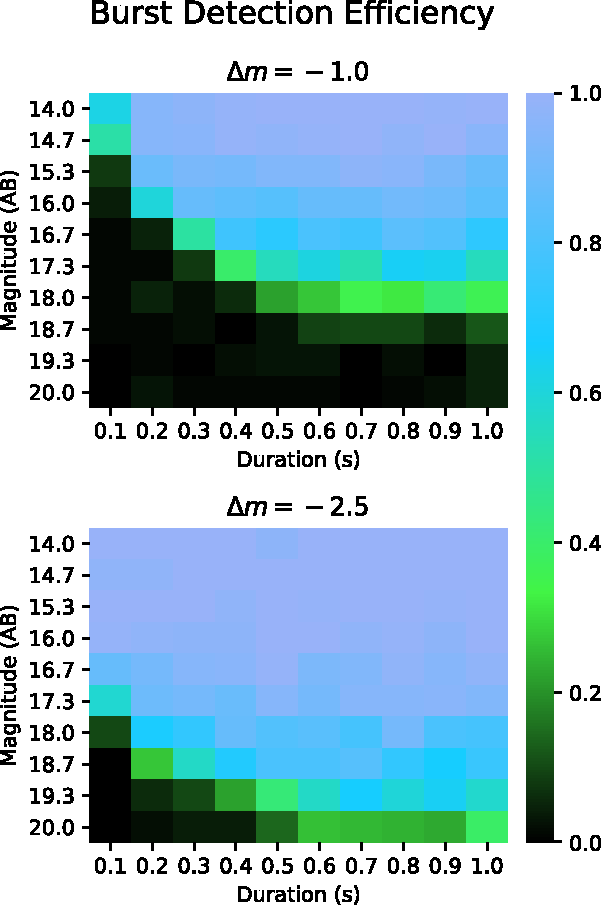
\includegraphics[width=\columnwidth]{f6.pdf}
% \caption{The burst detection efficiency heat maps of the combined network on never before seen variable images. Each test sample contains one burst with a specified source magnitude and burst duration drawn from the $10 \times 10$ grid. The efficiency surfaces are interpolated from the efficiency values over the grid. The plots on the top and bottom correspond to sources with burst magnitude changes of -1.0 and -2.5 respectively.}
% % http://localhost:8888/notebooks/Code/Astronomy/exp4/notebooks/Test4Results_20180517-Copy1.ipynb
% \label{fig:6}
% \end{figure}

\begin{figure*}[htb]
\center
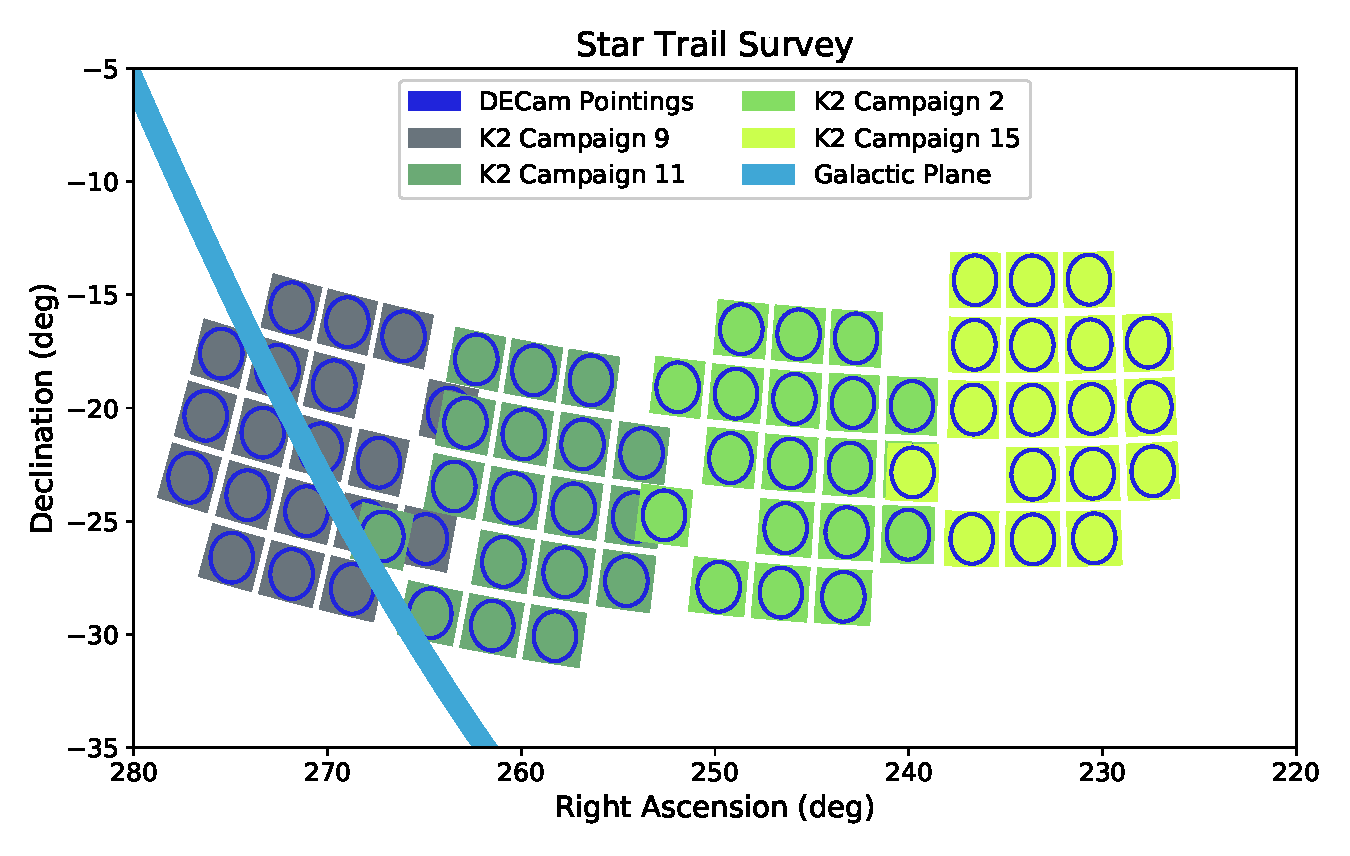
\includegraphics[width=\columnwidth]{survey.eps}
\caption{The proposed 270 degree star trail survey. The four K2 fields are shown in varying shades of green. Each DECam pointing will inscribe a single Kepler module of 4 CCDs. The first pass will take static exposures; the remaining two passes will take star trail exposures.}
\label{fig:1}
\end{figure*}

\begin{figure*}[htb]
\center
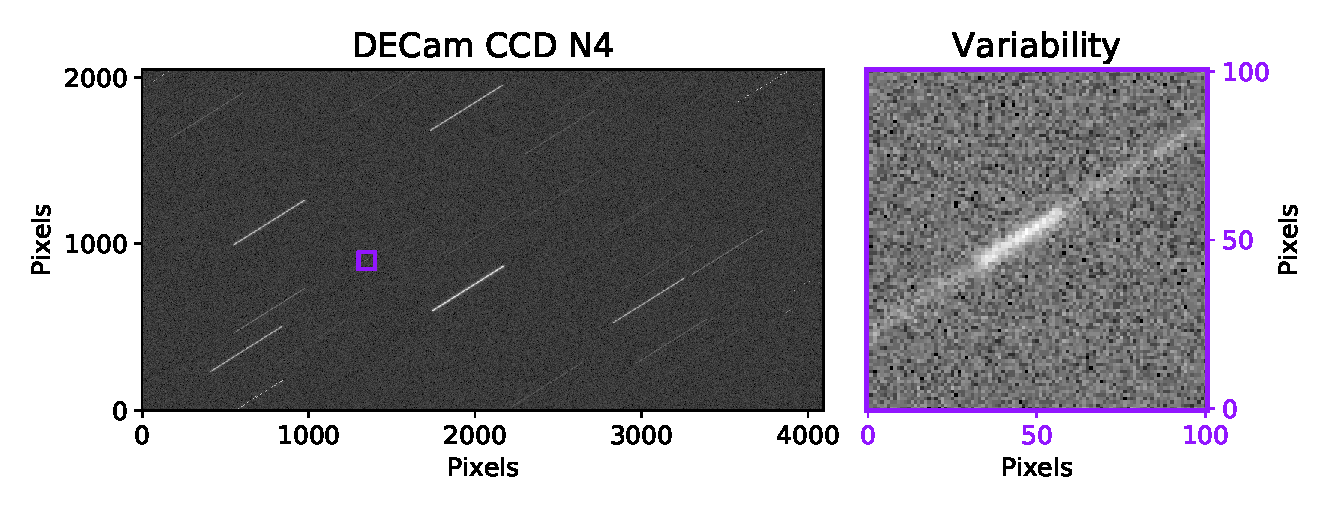
\includegraphics[width=\columnwidth]{decamtrails.eps}
\caption{\textit{Left:} A simulated DECam star trail image on the N4 CCD. The region exhibiting variability is outlined in purple. \textit{Right:} A 100 x 100 pixel crop and zoom-in of the variable region.}
\label{fig:2}
\end{figure*}

\begin{figure*}[htb]
\center
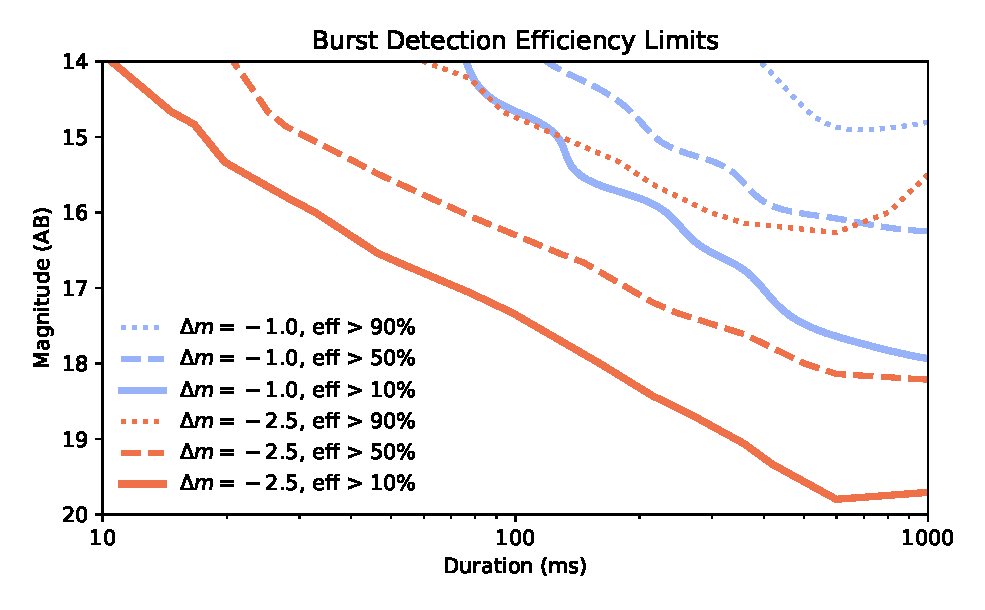
\includegraphics[width=\columnwidth]{contour.eps}
\caption{The contours show the probability the network will detect a burst with the given source magnitude and burst duration. The blue and red contours correspond to burst magnitude changes of -1.0 and -2.5 respectively. The dotted, dashed, and solid lines correspond to 90\%, 50\% and 10\% detection efficiencies respectively.}
\label{fig:3}
\end{figure*}


\clearpage

% EXPERIMENTAL DESIGN
%
% This section should consist of text only (no figures).
% There is a limit of one page of printed text.

% Describe your overall observational program.  How will these 
% observations contribute toward the accomplishment of the goals 
% outlined in the science justification?  If you've requested 
% long-term status, justify why this is necessary for successful 
% completion of the science.
%
% NOTE: In previous versions of the proposal form, this section
% requested details about the use of non-NOAO observing facilities. 
% Such information should now be entered in the following "Other
% Facilities" section.

\expdesign
% for decam cite (Flaugher et. al 2015)
% 20s readout time
\subsection*{Observing Four Adjacent K2 Campaigns: 2,9,11,15}

The Kepler K2 mission is a sequence of continuous 80-day observing campaigns of fields distributed around the ecliptic plane. Each field contains thousands of targets with well-characterized optical light curves, many with 2-minute cadence. This rich time-domain data makes these fields ideal for testing our method.

% This rich data has compelled astronomers to image these fields extensively, including in the near infrared and x-ray regimes. The constituents of these fields are well known, making them excellent targets to validate our method on. Furthermore, the analysis of any rare events we uncover will benefit from the wealth of existing data.

The survey we propose covers four K2 fields: 2,9,11,15. These adjacent fields extend from the galactic plane to 35 degrees above it, providing a wide range of source densities for our method. The fields in this suite also share good observing periods and can be surveyed in a single evening.

The DECam field of view almost perfectly inscribes a single Kepler Module of four CCDs. This allows us to efficiently cover the K2 fields by visiting the center locations of the modules. We tile each field 3 times in the `r' band. The first is a static exposure for reference. The following two visits take 15 second star trail exposures. We discuss these choices further in the technical description. 

\subsection*{Image Processing and Analysis}

The image processing and analysis has three stages. First we generate simulated data and train the algorithm on it. We will use the Sherlock 2.0 high performance computing cluster at Stanford University to produce a suite of simulated DECam star trail images. CatSim will be used to seed realistic catalogs; PhoSim, which has already been used to study DECam, will be used for the image simulations. Then we will train networks to detect three variable signatures: bursts, occultations, and smooth trends on timescales of tens of milliseconds to minutes.

In the second stage we calibrate the performance of the algorithm. We will insert simulated variable star trails in the real DECam images and examine the algorithm's ability to uncover them. If we discover effects in the DECam images that are not captured in the simulations, then we can set aside a partition of the real data to use in the training, which will push the network to generalize. At the end of this stage we will have established consistent performance on simulated and real images and have measured the algorithm's performance limits on the signatures of interest.

The third stage will be scanning the real DECam data and communicating the results. The variable events we find will collectively support global statistical analysis and individually be candidates for custom, detailed follow-up analysis. We will combine the variable events with the performance limits to constrain the frequency of specific short duration phenomena in our galaxy. 

% PROPRIETARY PERIOD
% 
% Enter the proprietary period for your data between the braces.
% The normal duration is 18 months from when the data are taken at
% the telescope.  Requests for longer proprietary periods must
% be approved by the NOAO Director.

\proprietaryperiod{18 months}


% OTHER FACILITIES OR RESOURCES
% 
% This section should consist of text only (no figures).
% Please limit to about a half page of printed text.
% 
% 1) We are interested in understanding how observations made through
% NOAO observing opportunities complement or support data from other
% facilities both on the ground and in space.   We will use this
% information to guide the evolution of the NOAO program; it will not
% affect the success of your proposal in the evaluation process.
% Please describe how the proposed observations complement data from  
% other facilities, including private observatories and both ground-
% and space-based telescopes.  In addressing this question, take a
% broad view of your research program.  Are the data to be obtained 
% through this proposal going to help select samples for detailed
% observations using larger telescopes or from space observatories?
% Are these data going to be directly combined with data obtained
% elsewhere to test a hypothesis?  Will these observations have
% relevance to other observations, even though the proposal stands
% on its own?  For each of these other facilities, indicate the nature
% of the observations (yours or those of others), and describe the
% importance of the observations proposed here in the context of the
% entire program.
%
% 2) Do you currently have a grant that would provide resources
% to support the data processing, analysis, and publication of the
% observations proposed here?

\otherfacilities

The proposed survey will provide high time resolution data on 270 square degrees of sky. This will complement multiple analyses already performed on the Kepler field that overlaps it, including ,, .

If this works well, then we can scale it up to the next generation ground-based wide field telescope: the LSST. The PI already is working on commissioning projects on the Telescope and Site team. He also has access to the Sherlock 2.0 computing cluster at Stanford University. This will fulfill our needs.

% LONG-TERM DETAILS
%
% If you are requesting long-term status for this proposal briefly 
% state the requirements for telescope time (telescope, instrument, 
% number of nights) needed in subsequent semesters to complete this 
% project in \longtermdetails (be sure to uncomment the 
% \longtermdetails line below).
%
% If this is a long-term request you MAY ALSO NEED to modify the
% \proposaltype keyword at the top of this form changing "Standard"
% to "Longterm" (where is says "Please do not modify or delete this 
% line!").  It is this keyword that will flag this proposal as a 
% long-term status request, regardless of what may be entered here 
% in \longtermdetails!
%
% If this is not a long-term status request then please ignore this
% section.
%
%
%\longtermdetails


% PAST USE
%
% How effectively have you used the facilities available through NOAO
% in the past?
% List allocations of telescope time on facilities available through 
% NOAO to the Principal Investigator during the past 2 years, together 
% with the current status of the data (cite publications where 
% appropriate).  Mark any allocations of time related to the current 
% proposal with a \relatedwork{} command.

\thepast

This will be the first time David Thomas observes at NOAO facilities. He is supported by a team that has ample experience with NOAO facilities including WIYN, Blanco, and the upcoming LSST. 

%%%%%%%%%%%%%%%%%%%%%%%%%%%%%%%%%%%%%%%%%%%%%%%%%%%%%%%%%%%%%%%%%%%%%%

% OBSERVING RUN DETAILS - REQUIRED FOR EACH OBSERVING RUN REQUESTED
%
% For each run requested earlier in the \begin{obsruns}-\end{obsruns}
% sections of this proposal form, further run information must be
% specified.  Enter this block of information for each non-Gemini run.

% The \runid field must contain the run number plus 
% telescope/instrument-detector information as it appears for each 
% run in the obsruns sections. For example, 
% \runid{1}{KP-4m/ECHUV + T2KB}.

\runid{1}{CT-4m/DECam}

% Describe the observations to be made during this observing run in
% the \technicaldescription section. Justify the specific telescope,
% the number of nights, the instrument, and the lunar phase requested.
% List objects, coordinates, and magnitudes (or surface brightness, if
% appropriate) using a LaTeX-coded table in this section or optionally
% enter the target information using the Target Tables described at
% the end of this template.  Target Tables of objects are required for 
% queue runs.
%
% Exposure time calculators (ETCs) for some optical and IR 
% instruments in use at CTIO and at KPNO are available to assist 
% you with the preparation of your proposal.  See the Web pages:
%    Imaging ETC      - http://www.noao.edu/gateway/ccdtime/
%    Spectroscopy ETC - http://www.noao.edu/gateway/spectime/

\technicaldescription

The crux of our experiment is to resolve star trails and detect changes in individual trails. We use four metrics to assess how the exposure time impacts these goals: trail resolution SNR ($S_{res}$), trail change SNR ($S_{change}$), CCD fraction ($C$), and survey duty cycle ($D$). $S_{res}$ compares the ratio of flux in the trail to the sky background, source Poisson, and readout noises. Contrary to conventional exposures, this ratio decreases with exposure time because once a trail passes over a pixel it stops providing signal to it, while the sky background continues to increase with time. $S_{change}$ compares the immediate change of flux a source to the sky background, source Poisson, and readout noises. $C$ is the ratio of the length of an equatorial star trail over the length of the diagonal of a 2048 x 4096 pixel DECam CCD. It provides a sense of the fraction of sources that trail off CCDs. $D$ is the fraction of exposure time over the combined exposure-readout-slew-time and shows how efficient our survey is with its allocated time.

We use many variables from the \textit{DECam User Guide} in our metrics code, including zero-points, filter transmissions, readout noise, sky brightness, and slew time as a function of angle. We find that 15 second exposures in the `r' band are optimal for these metrics. These exposures give $S_{res} > 10$ for trails with source magnitudes $m < 14$. They also give $S_{change} > 5$ for $\Delta m = -0.2, m < 12.5$ or $\Delta m = -1.0, m < 15$. $C$ is 0.19, which roughly means that greater than 80\% of the trails are contained within the CCD. The average readout and slew time for our survey is 31 seconds leading to a reasonable duty cycle of $D = 0.33$.

We take three exposures of each target. The first is a 15 second static exposure and serves as a reference image which will be valuable to our testing and analysis. The final two are 15 second star trail exposures. Progressing through the four K2 fields will take around 3 hours and 8 minutes, which includes exposure, readout, and slew times. The remainder of the half-night is a safety buffer, which will allow us to address any issues that come up using the telescope in this unique manner. If we keep to the schedule and have sufficient time remaining, then we do one more pass over the fields.

There are three periods between May and July that are particularly favorable for our survey. The first half of the night from July 18 to 31; the second half of the night May 1 to 13; and the second half of the night from May 28 to June 5. All these nights have at least 3 hours where each field is at airmass $<$ 1.5 and limited moonlight. Finally, we have confirmed that our targets are within the Blanco 4-m/DECam horizon limits.


% In the tech desc can you say what S/N you will get as a function of source magnitude and say how many variable sources you expect in the Kepler fields. What S/N is required for a good detection?

% \begin{itemize}
% 	\item We used JSkyCalc to confirm there are good dates between May-July where all fields can be observed through a reasonable airmass. 
% 	\item Confirmed survey is within Blanco 4-m horizon limites.
% 	\item Survey should take 3 hours and 8 minutes in theory, which leaves a buffer of approximately 2 hours.
% 	\item We used DECam zero-magnitude and filter throughput data to model the signal to noise ratio. The choice of 15 second exposures is guided by 3 effects: background noise increases while signal is constant after source trails through so after a few 100 milliseconds SNR $\sim 1/\sqrt(t_{exp})$, we don't want trails to be significant portion of CCD, and we want a reasonable duty cycle given almost 20 second readout time. 
% \end{itemize}

% Several instrument configuration parameters are requested.  Fill
% these in as appropriate for each run. 
%
% \begin{configuration}
% \filters{}            % List here any filters that you plan to use.
% \grating{}            % List any gratings/grisms need with this run.
% \order{}              % Specify any grating order(s).
% \crossdisperser{}     % List cross disperser, if needed.
% \slit{}               % Enter slit widths you plan to use.
% \multislit{}          % yes or no only
% \wstart{}             % Starting wavelength of wavelength range.
% \wend{}               % Ending wavelength of wavelength range.
% \cable{}              % For CTIO/Hydra: enter 2.0".  For WIYN: enter
%                         red, blue, or densepak.
% \corrector{}          % Enter red or blue for KP-coude, CAM5.
% \collimator{}         % Enter collimator needed.
% \adc{}                % If user selectable, enter yes or no only.
% \end{configuration}
%
% Details about these fields are available in the online help for the
% Web form at http://www.noao.edu/noaoprop/help/standard.html#iconfig

\begin{configuration}
\filters{r}
\grating{-}
\order{-}
\crossdisperser{-}       
\slit{-}
\multislit{-}            
\wstart{-}
\wend{-}
\cable{-}
\corrector{-}            
\collimator{-}             
\adc{-}
\end{configuration}
\newpage
\begin{center}
\begin{longtable}{|c|c|c|c|c|c|}
\hline
RA (deg)& Dec (deg)& Filter & Tracking & Exposure Time (sec) & Comment\\
\hline
263.72779 & -20.201175 & r & on &15 & K2 Campaign-9, Module-1\\
264.9247 & -25.784213 & r & on &15 & K2 Campaign-9, Module-3\\
266.07655 & -16.82745 & r & on &15 & K2 Campaign-9, Module-4\\
267.34745 & -22.412586 & r & on &15 & K2 Campaign-9, Module-6\\
268.0217 & -25.201351 & r & on &15 & K2 Campaign-9, Module-7\\
268.72661 & -27.984544 & r & on &15 & K2 Campaign-9, Module-8\\
268.97252 & -16.209388 & r & on &15 & K2 Campaign-9, Module-9\\
269.65253 & -18.992061 & r & on &15 & K2 Campaign-9, Module-10\\
270.35534 & -21.774739 & r & on &15 & K2 Campaign-9, Module-11\\
271.08764 & -24.552602 & r & on &15 & K2 Campaign-9, Module-12\\
271.85166 & -27.328437 & r & on &15 & K2 Campaign-9, Module-13\\
271.8502 & -15.549016 & r & on &15 & K2 Campaign-9, Module-14\\
272.58167 & -18.316964 & r & on &15 & K2 Campaign-9, Module-15\\
273.33749 & -21.082731 & r & on &15 & K2 Campaign-9, Module-16\\
274.12191 & -23.844644 & r & on &15 & K2 Campaign-9, Module-17\\
274.93987 & -26.602962 & r & on &15 & K2 Campaign-9, Module-18\\
275.48614 & -17.597012 & r & on &15 & K2 Campaign-9, Module-19\\
276.2882 & -20.33974 & r & on &15 & K2 Campaign-9, Module-20\\
277.12054 & -23.077546 & r & on &15 & K2 Campaign-9, Module-21\\
263.72779 & -20.201175 & r & off &15 & K2 Campaign-9, Module-1\\
264.9247 & -25.784213 & r & off &15 & K2 Campaign-9, Module-3\\
266.07655 & -16.82745 & r & off &15 & K2 Campaign-9, Module-4\\
267.34745 & -22.412586 & r & off &15 & K2 Campaign-9, Module-6\\
268.0217 & -25.201351 & r & off &15 & K2 Campaign-9, Module-7\\
268.72661 & -27.984544 & r & off &15 & K2 Campaign-9, Module-8\\
268.97252 & -16.209388 & r & off &15 & K2 Campaign-9, Module-9\\
269.65253 & -18.992061 & r & off &15 & K2 Campaign-9, Module-10\\
270.35534 & -21.774739 & r & off &15 & K2 Campaign-9, Module-11\\
271.08764 & -24.552602 & r & off &15 & K2 Campaign-9, Module-12\\
271.85166 & -27.328437 & r & off &15 & K2 Campaign-9, Module-13\\
271.8502 & -15.549016 & r & off &15 & K2 Campaign-9, Module-14\\
272.58167 & -18.316964 & r & off &15 & K2 Campaign-9, Module-15\\
273.33749 & -21.082731 & r & off &15 & K2 Campaign-9, Module-16\\
274.12191 & -23.844644 & r & off &15 & K2 Campaign-9, Module-17\\
274.93987 & -26.602962 & r & off &15 & K2 Campaign-9, Module-18\\
275.48614 & -17.597012 & r & off &15 & K2 Campaign-9, Module-19\\
276.2882 & -20.33974 & r & off &15 & K2 Campaign-9, Module-20\\
277.12054 & -23.077546 & r & off &15 & K2 Campaign-9, Module-21\\
263.72779 & -20.201175 & r & off &15 & K2 Campaign-9, Module-1\\
264.9247 & -25.784213 & r & off &15 & K2 Campaign-9, Module-3\\
266.07655 & -16.82745 & r & off &15 & K2 Campaign-9, Module-4\\
267.34745 & -22.412586 & r & off &15 & K2 Campaign-9, Module-6\\
268.0217 & -25.201351 & r & off &15 & K2 Campaign-9, Module-7\\
268.72661 & -27.984544 & r & off &15 & K2 Campaign-9, Module-8\\
268.97252 & -16.209388 & r & off &15 & K2 Campaign-9, Module-9\\
269.65253 & -18.992061 & r & off &15 & K2 Campaign-9, Module-10\\
270.35534 & -21.774739 & r & off &15 & K2 Campaign-9, Module-11\\
271.08764 & -24.552602 & r & off &15 & K2 Campaign-9, Module-12\\
271.85166 & -27.328437 & r & off &15 & K2 Campaign-9, Module-13\\
271.8502 & -15.549016 & r & off &15 & K2 Campaign-9, Module-14\\
272.58167 & -18.316964 & r & off &15 & K2 Campaign-9, Module-15\\
273.33749 & -21.082731 & r & off &15 & K2 Campaign-9, Module-16\\
274.12191 & -23.844644 & r & off &15 & K2 Campaign-9, Module-17\\
274.93987 & -26.602962 & r & off &15 & K2 Campaign-9, Module-18\\
275.48614 & -17.597012 & r & off &15 & K2 Campaign-9, Module-19\\
276.2882 & -20.33974 & r & off &15 & K2 Campaign-9, Module-20\\
277.12054 & -23.077546 & r & off &15 & K2 Campaign-9, Module-21\\
267.17021 & -25.669376 & r & on &15 & K2 Campaign-11, Module-1\\
264.69931 & -29.064482 & r & on &15 & K2 Campaign-11, Module-4\\
263.45917 & -23.462254 & r & on &15 & K2 Campaign-11, Module-6\\
262.87765 & -20.656998 & r & on &15 & K2 Campaign-11, Module-7\\
262.31833 & -17.852577 & r & on &15 & K2 Campaign-11, Module-8\\
261.49601 & -29.605946 & r & on &15 & K2 Campaign-11, Module-9\\
260.92737 & -26.79314 & r & on &15 & K2 Campaign-11, Module-10\\
260.38681 & -23.975597 & r & on &15 & K2 Campaign-11, Module-11\\
259.86765 & -21.157819 & r & on &15 & K2 Campaign-11, Module-12\\
259.36942 & -18.336932 & r & on &15 & K2 Campaign-11, Module-13\\
258.25987 & -30.072995 & r & on &15 & K2 Campaign-11, Module-14\\
257.76264 & -27.251584 & r & on &15 & K2 Campaign-11, Module-15\\
257.28983 & -24.428065 & r & on &15 & K2 Campaign-11, Module-16\\
256.83751 & -21.60315 & r & on &15 & K2 Campaign-11, Module-17\\
256.40292 & -18.776225 & r & on &15 & K2 Campaign-11, Module-18\\
254.57518 & -27.639373 & r & on &15 & K2 Campaign-11, Module-19\\
254.17478 & -24.816517 & r & on &15 & K2 Campaign-11, Module-20\\
253.79079 & -21.993558 & r & on &15 & K2 Campaign-11, Module-21\\
267.17021 & -25.669376 & r & off &15 & K2 Campaign-11, Module-1\\
264.69931 & -29.064482 & r & off &15 & K2 Campaign-11, Module-4\\
263.45917 & -23.462254 & r & off &15 & K2 Campaign-11, Module-6\\
262.87765 & -20.656998 & r & off &15 & K2 Campaign-11, Module-7\\
262.31833 & -17.852577 & r & off &15 & K2 Campaign-11, Module-8\\
261.49601 & -29.605946 & r & off &15 & K2 Campaign-11, Module-9\\
260.92737 & -26.79314 & r & off &15 & K2 Campaign-11, Module-10\\
260.38681 & -23.975597 & r & off &15 & K2 Campaign-11, Module-11\\
259.86765 & -21.157819 & r & off &15 & K2 Campaign-11, Module-12\\
259.36942 & -18.336932 & r & off &15 & K2 Campaign-11, Module-13\\
258.25987 & -30.072995 & r & off &15 & K2 Campaign-11, Module-14\\
257.76264 & -27.251584 & r & off &15 & K2 Campaign-11, Module-15\\
257.28983 & -24.428065 & r & off &15 & K2 Campaign-11, Module-16\\
256.83751 & -21.60315 & r & off &15 & K2 Campaign-11, Module-17\\
256.40292 & -18.776225 & r & off &15 & K2 Campaign-11, Module-18\\
254.57518 & -27.639373 & r & off &15 & K2 Campaign-11, Module-19\\
254.17478 & -24.816517 & r & off &15 & K2 Campaign-11, Module-20\\
253.79079 & -21.993558 & r & off &15 & K2 Campaign-11, Module-21\\
267.17021 & -25.669376 & r & off &15 & K2 Campaign-11, Module-1\\
264.69931 & -29.064482 & r & off &15 & K2 Campaign-11, Module-4\\
263.45917 & -23.462254 & r & off &15 & K2 Campaign-11, Module-6\\
262.87765 & -20.656998 & r & off &15 & K2 Campaign-11, Module-7\\
262.31833 & -17.852577 & r & off &15 & K2 Campaign-11, Module-8\\
261.49601 & -29.605946 & r & off &15 & K2 Campaign-11, Module-9\\
260.92737 & -26.79314 & r & off &15 & K2 Campaign-11, Module-10\\
260.38681 & -23.975597 & r & off &15 & K2 Campaign-11, Module-11\\
259.86765 & -21.157819 & r & off &15 & K2 Campaign-11, Module-12\\
259.36942 & -18.336932 & r & off &15 & K2 Campaign-11, Module-13\\
258.25987 & -30.072995 & r & off &15 & K2 Campaign-11, Module-14\\
257.76264 & -27.251584 & r & off &15 & K2 Campaign-11, Module-15\\
257.28983 & -24.428065 & r & off &15 & K2 Campaign-11, Module-16\\
256.83751 & -21.60315 & r & off &15 & K2 Campaign-11, Module-17\\
256.40292 & -18.776225 & r & off &15 & K2 Campaign-11, Module-18\\
254.57518 & -27.639373 & r & off &15 & K2 Campaign-11, Module-19\\
254.17478 & -24.816517 & r & off &15 & K2 Campaign-11, Module-20\\
253.79079 & -21.993558 & r & off &15 & K2 Campaign-11, Module-21\\
252.62898 & -24.737815 & r & on &15 & K2 Campaign-2, Module-1\\
251.92999 & -19.084268 & r & on &15 & K2 Campaign-2, Module-3\\
249.8097 & -27.893175 & r & on &15 & K2 Campaign-2, Module-4\\
249.20516 & -22.208053 & r & on &15 & K2 Campaign-2, Module-6\\
248.92019 & -19.36398 & r & on &15 & K2 Campaign-2, Module-7\\
248.64576 & -16.522263 & r & on &15 & K2 Campaign-2, Module-8\\
246.60037 & -28.147494 & r & on &15 & K2 Campaign-2, Module-9\\
246.35669 & -25.298709 & r & on &15 & K2 Campaign-2, Module-10\\
246.125 & -22.447025 & r & on &15 & K2 Campaign-2, Module-11\\
245.90076 & -19.596442 & r & on &15 & K2 Campaign-2, Module-12\\
245.68598 & -16.744145 & r & on &15 & K2 Campaign-2, Module-13\\
243.37691 & -28.329937 & r & on &15 & K2 Campaign-2, Module-14\\
243.20141 & -25.47929 & r & on &15 & K2 Campaign-2, Module-15\\
243.03384 & -22.627974 & r & on &15 & K2 Campaign-2, Module-16\\
242.8729 & -19.7765 & r & on &15 & K2 Campaign-2, Module-17\\
242.71813 & -16.924105 & r & on &15 & K2 Campaign-2, Module-18\\
240.03962 & -25.593367 & r & on &15 & K2 Campaign-2, Module-19\\
239.93857 & -22.749248 & r & on &15 & K2 Campaign-2, Module-20\\
239.84013 & -19.90586 & r & on &15 & K2 Campaign-2, Module-21\\
252.62898 & -24.737815 & r & off &15 & K2 Campaign-2, Module-1\\
251.92999 & -19.084268 & r & off &15 & K2 Campaign-2, Module-3\\
249.8097 & -27.893175 & r & off &15 & K2 Campaign-2, Module-4\\
249.20516 & -22.208053 & r & off &15 & K2 Campaign-2, Module-6\\
248.92019 & -19.36398 & r & off &15 & K2 Campaign-2, Module-7\\
248.64576 & -16.522263 & r & off &15 & K2 Campaign-2, Module-8\\
246.60037 & -28.147494 & r & off &15 & K2 Campaign-2, Module-9\\
246.35669 & -25.298709 & r & off &15 & K2 Campaign-2, Module-10\\
246.125 & -22.447025 & r & off &15 & K2 Campaign-2, Module-11\\
245.90076 & -19.596442 & r & off &15 & K2 Campaign-2, Module-12\\
245.68598 & -16.744145 & r & off &15 & K2 Campaign-2, Module-13\\
243.37691 & -28.329937 & r & off &15 & K2 Campaign-2, Module-14\\
243.20141 & -25.47929 & r & off &15 & K2 Campaign-2, Module-15\\
243.03384 & -22.627974 & r & off &15 & K2 Campaign-2, Module-16\\
242.8729 & -19.7765 & r & off &15 & K2 Campaign-2, Module-17\\
242.71813 & -16.924105 & r & off &15 & K2 Campaign-2, Module-18\\
240.03962 & -25.593367 & r & off &15 & K2 Campaign-2, Module-19\\
239.93857 & -22.749248 & r & off &15 & K2 Campaign-2, Module-20\\
239.84013 & -19.90586 & r & off &15 & K2 Campaign-2, Module-21\\
252.62898 & -24.737815 & r & off &15 & K2 Campaign-2, Module-1\\
251.92999 & -19.084268 & r & off &15 & K2 Campaign-2, Module-3\\
249.8097 & -27.893175 & r & off &15 & K2 Campaign-2, Module-4\\
249.20516 & -22.208053 & r & off &15 & K2 Campaign-2, Module-6\\
248.92019 & -19.36398 & r & off &15 & K2 Campaign-2, Module-7\\
248.64576 & -16.522263 & r & off &15 & K2 Campaign-2, Module-8\\
246.60037 & -28.147494 & r & off &15 & K2 Campaign-2, Module-9\\
246.35669 & -25.298709 & r & off &15 & K2 Campaign-2, Module-10\\
246.125 & -22.447025 & r & off &15 & K2 Campaign-2, Module-11\\
245.90076 & -19.596442 & r & off &15 & K2 Campaign-2, Module-12\\
245.68598 & -16.744145 & r & off &15 & K2 Campaign-2, Module-13\\
243.37691 & -28.329937 & r & off &15 & K2 Campaign-2, Module-14\\
243.20141 & -25.47929 & r & off &15 & K2 Campaign-2, Module-15\\
243.03384 & -22.627974 & r & off &15 & K2 Campaign-2, Module-16\\
242.8729 & -19.7765 & r & off &15 & K2 Campaign-2, Module-17\\
242.71813 & -16.924105 & r & off &15 & K2 Campaign-2, Module-18\\
240.03962 & -25.593367 & r & off &15 & K2 Campaign-2, Module-19\\
239.93857 & -22.749248 & r & off &15 & K2 Campaign-2, Module-20\\
239.84013 & -19.90586 & r & off &15 & K2 Campaign-2, Module-21\\
239.80112 & -22.842778 & r & on &15 & K2 Campaign-15, Module-1\\
236.74854 & -25.77599 & r & on &15 & K2 Campaign-15, Module-4\\
236.66006 & -20.065128 & r & on &15 & K2 Campaign-15, Module-6\\
236.61699 & -17.208912 & r & on &15 & K2 Campaign-15, Module-7\\
236.57571 & -14.355501 & r & on &15 & K2 Campaign-15, Module-8\\
233.58956 & -25.795758 & r & on &15 & K2 Campaign-15, Module-9\\
233.60258 & -22.938687 & r & on &15 & K2 Campaign-15, Module-10\\
233.61604 & -20.079162 & r & on &15 & K2 Campaign-15, Module-11\\
233.62703 & -17.220917 & r & on &15 & K2 Campaign-15, Module-12\\
233.63942 & -14.361349 & r & on &15 & K2 Campaign-15, Module-13\\
230.42998 & -25.750422 & r & on &15 & K2 Campaign-15, Module-14\\
230.50193 & -22.89622 & r & on &15 & K2 Campaign-15, Module-15\\
230.57069 & -20.041484 & r & on &15 & K2 Campaign-15, Module-16\\
230.63687 & -17.186745 & r & on &15 & K2 Campaign-15, Module-17\\
230.70161 & -14.331263 & r & on &15 & K2 Campaign-15, Module-18\\
227.40562 & -22.794871 & r & on &15 & K2 Campaign-15, Module-19\\
227.53054 & -19.951623 & r & on &15 & K2 Campaign-15, Module-20\\
227.64949 & -17.108981 & r & on &15 & K2 Campaign-15, Module-21\\
239.80112 & -22.842778 & r & off &15 & K2 Campaign-15, Module-1\\
236.74854 & -25.77599 & r & off &15 & K2 Campaign-15, Module-4\\
236.66006 & -20.065128 & r & off &15 & K2 Campaign-15, Module-6\\
236.61699 & -17.208912 & r & off &15 & K2 Campaign-15, Module-7\\
236.57571 & -14.355501 & r & off &15 & K2 Campaign-15, Module-8\\
233.58956 & -25.795758 & r & off &15 & K2 Campaign-15, Module-9\\
233.60258 & -22.938687 & r & off &15 & K2 Campaign-15, Module-10\\
233.61604 & -20.079162 & r & off &15 & K2 Campaign-15, Module-11\\
233.62703 & -17.220917 & r & off &15 & K2 Campaign-15, Module-12\\
233.63942 & -14.361349 & r & off &15 & K2 Campaign-15, Module-13\\
230.42998 & -25.750422 & r & off &15 & K2 Campaign-15, Module-14\\
230.50193 & -22.89622 & r & off &15 & K2 Campaign-15, Module-15\\
230.57069 & -20.041484 & r & off &15 & K2 Campaign-15, Module-16\\
230.63687 & -17.186745 & r & off &15 & K2 Campaign-15, Module-17\\
230.70161 & -14.331263 & r & off &15 & K2 Campaign-15, Module-18\\
227.40562 & -22.794871 & r & off &15 & K2 Campaign-15, Module-19\\
227.53054 & -19.951623 & r & off &15 & K2 Campaign-15, Module-20\\
227.64949 & -17.108981 & r & off &15 & K2 Campasdign-15, Module-21\\
239.80112 & -22.842778 & r & off &15 & K2 Campaign-15, Module-1\\
236.74854 & -25.77599 & r & off &15 & K2 Campaign-15, Module-4\\
236.66006 & -20.065128 & r & off &15 & K2 Campaign-15, Module-6\\
236.61699 & -17.208912 & r & off &15 & K2 Campaign-15, Module-7\\
236.57571 & -14.355501 & r & off &15 & K2 Campaign-15, Module-8\\
233.58956 & -25.795758 & r & off &15 & K2 Campaign-15, Module-9\\
233.60258 & -22.938687 & r & off &15 & K2 Campaign-15, Module-10\\
233.61604 & -20.079162 & r & off &15 & K2 Campaign-15, Module-11\\
233.62703 & -17.220917 & r & off &15 & K2 Campaign-15, Module-12\\
233.63942 & -14.361349 & r & off &15 & K2 Campaign-15, Module-13\\
230.42998 & -25.750422 & r & off &15 & K2 Campaign-15, Module-14\\
230.50193 & -22.89622 & r & off &15 & K2 Campaign-15, Module-15\\
230.57069 & -20.041484 & r & off &15 & K2 Campaign-15, Module-16\\
230.63687 & -17.186745 & r & off &15 & K2 Campaign-15, Module-17\\
230.70161 & -14.331263 & r & off &15 & K2 Campaign-15, Module-18\\
227.40562 & -22.794871 & r & off &15 & K2 Campaign-15, Module-19\\
227.53054 & -19.951623 & r & off &15 & K2 Campaign-15, Module-20\\
227.64949 & -17.108981 & r & off &15 & K2 Campaign-15, Module-21\\
\hline
\end{longtable}
\end{center}

% \begin{targettable}{Run 1: CT-4m/DECam}
% \objid{1,2}           % specify a 3-digit number for each target
% \object{1}          % 20 characters maximum
% \ra{1}              % e.g., xx:xx:xx.x
% \dec{1}             % e.g., +-xx:xx:xx.x
% \epoch{1}           % e.g., 1950.3
% \magnitude{1}
% \filter{1}
% \exptime{1}         % in seconds PER EXPOSURE
% \nexposures{1}      % Number of exposures
% \moondays{1}        % Days from new moon, use a number 0-14
% \skycond{1}         % "spec" or "phot"
% \seeing{1}          % max allowable PSF FWHM (arcsecs)
% \obscomment{1}      % 20 characters maximum - REQUIRED COMMAND
%  % - repeat target entry parameters as needed to complete Table -
% \end{targettable}



% COORDINATE RANGES OF PRINCIPLE TARGETS   
% Use the \targetsra and \targetsdec fields to specify the range
% of right ascension (in hours) and declination (in degrees) of your
% principle targets for this observing run.
%
% For example:
%
%  \targetsra{14 to 17}
%  \targetsdec{-10 to 35}

\targetsra{3.31 hours}			% RA range in hours
\targetsdec{15.74 degrees}			% Dec. range in degrees



% Use \specialrequest to describe briefly any special or non-standard
% usage of instrumentation. 
\specialrequest

We have discussed using the Blanco telescope and DECam in non-tracking mode with the Blanco Instrument Scientist Dr. Alistair Walker. Dr. Walker believes the taking of trailed images can be automated through the DECam instrument control system, SISPI, which sends commands to the Blanco Telescope Control System. We will work with CTIO to develop and test this capability if our proposal is successful. Working with the telescope operator to manually toggle between tracking and non-tracking will be our back up plan.

% If you plan to submit any Target Tables for this run they must be
% entered here.  Target Tables are required for all queue runs.

% TARGET TABLES
%
% Target Tables are required for all queue runs and are
% are optional for classically scheduled runs.  Target
% Tables, if included, are associated with each run in the observing
% run details section of the proposal form and must follow the 
% \specialrequest in each section.
%
% CT-1.3m tables require that all the fields in the target table be
% specified.  For other tables specific fields may be deleted EXCEPT 
% for the \obscomment command as mentioned below.
%
% Queue investigators should supply good coordinates
% with the \ra and \dec commands since these values may be used to
% observe your fields.
%
% Note that for iterative targets, only the parameters that need
% to be changed have to be specified.  Once a parameter is specified in
% a targettable environment, it is retained until explicitly changed.
%
% The \obscomment command is REQUIRED for each target entry and
% must be the last item; this command forces each target line to be
% printed.  If no comment is needed, leave the argument blank.
%
% The \begin{targettable}{} command for each table must contain the
% telescope/instrument-detector information for that particular run,
% i.e,. \begin{targettable}{KP-4m/ECHUV + T2KB}.
%
% HINTS: Long tables do not break across pages. If it is necessary to
% continue a table across a page you must start a new table.  Use
% /clearpage before the \begin{targettable} command for the new table.
%
%\begin{targettable}{}
%\objid{}           % specify a 3-digit number for each target.
%\object{}          % 20 characters maximum
%\ra{}              % e.g., xx:xx:xx.x
%\dec{}             % e.g., +-xx:xx:xx.x
%\epoch{}           % e.g., 1950.3
%\magnitude{}
%\filter{}
%\exptime{}         % in seconds PER EXPOSURE
%\nexposures{}      % Number of exposures
%\moondays{}        % Days from new moon, use a number 0-14
%\skycond{}         % "spec" or "phot"
%\seeing{}          % max allowable PSF FWHM (arcsecs)
%\obscomment{}      % 20 characters maximum - REQUIRED COMMAND
%  - repeat target entry parameters as needed to complete Table -
%\end{targettable}


%%%%%%%%%%%%%%%%%%%%%%%%%%%%%%%%%%%%%%%%%%%%%%%%%%%%%%%%%%%%%%%%%%

% Detailed information as noted below must be provided for all runs 
% up to SIX runs.  Since Gemini runs must be specified through the 
% Web form this section only applies to non-Gemini runs - use the 
% Web form to generate detailed information and target tables for 
% Gemini runs.  Target Tables are required for queue runs but
% are optional for classical observing.
%
% \runid{}{}
% \technicaldescription
% \begin{configuration}
% \filters{r,i}
% \grating{NA}
% \order{NA}
% \crossdisperser{NA}
% \slit{NA}
% \multislit{NA}
% \wstart{NA}
% \wend{NA}
% \cable{NA}
% \corrector{NA}
% \collimator{NA}
% \adc{NA}
% \end{configuration}
% \specialrequest    % remove and not use for HET runs

\bibliographystyle{aasjournal}
\bibliography{references}

%%%%%%%%%%%%%%%%%%%%%%%%%%%%%%%%%%%%%%%%%%%%%%%%%%%%%%%%%%%%%%%%%%

% Please do not modify or delete this line.
\end{document}

% PROPOSAL SUBMISSION (if not submitting from the online proposal form):
%
%
% Upload this completed proposal latex file and figures at: 
%            https://www.noao.edu/noaoprop/submit/
%
%
% Thank you for your interest in NOAO.  Contact us at
% noaoprop-help@noao.edu if you have any suggestions or comments.
